\documentclass[openbib]{article}

\usepackage{color}
\usepackage{ctex}
\usepackage{mathtools}
\usepackage{amsmath}
\usepackage{graphicx,psfrag,epsfig}
% Copyright 20120 Liutao Tian, MIT License
% https://github.com/andy123t/code-latex-style/

\usepackage{listings,color}

% Matlab highlight color settings
%\definecolor{mBasic}{RGB}{248,248,242}       % default
\definecolor{mKeyword}{RGB}{0,0,255}          % bule
\definecolor{mString}{RGB}{160,32,240}        % purple
\definecolor{mComment}{RGB}{34,139,34}        % green
\definecolor{mBackground}{RGB}{245,245,245}   % lightgrey
\definecolor{mNumber}{RGB}{134,145,148}       % gray

\definecolor{Numberbg}{RGB}{237,240,241}     % lightgrey

% Python highlight color settings
%\definecolor{pBasic}{RGB}{248, 248, 242}     % default
\definecolor{pKeyword}{RGB}{228,0,128}        % magenta
\definecolor{pString}{RGB}{148,0,209}         % purple
\definecolor{pComment}{RGB}{117,113,94}       % gray
\definecolor{pIdentifier}{RGB}{166, 226, 46}  %
\definecolor{pBackground}{RGB}{245,245,245}   % lightgrey
\definecolor{pNumber}{RGB}{134,145,148}       % gray

\lstnewenvironment{Python}[1]{
	\lstset{language=python,               % choose the language of the code
		xleftmargin=30pt,
		xrightmargin=10pt,
		frame=l,
		framesep=15pt,%framerule=0pt,  % sets the frame style
		%frame=shadowbox,rulesepcolor=\color{red!20!green!20!blue!20},
		%basicstyle=\small\ttfamily,          % sets font style for the code
		basicstyle=\footnotesize\fontspec{Consolas},
		keywordstyle=\color{pKeyword},       % sets color for keywords
		stringstyle=\color{pString},         % sets color for strings
		commentstyle=\color{pComment},       % sets color for comments
		backgroundcolor=\color{pBackground}, % choose the background color
		title=#1,                            %\lstname show the filename of files
		emph={format_string,eff_ana_bf,permute,eff_ana_btr},
		emphstyle=\color{pIdentifier}
		showspaces=false,                    % show spaces adding particular underscores
		showstringspaces=false,              % underline spaces within strings
		showtabs=false,                      % show tabs within strings adding particular underscores
		tabsize=4,                           % sets default tabsize to 2 spaces
		captionpos=t,                        % sets the caption-position to bottom
		breaklines=true,                     % sets automatic line breaking
		framexleftmargin=5pt,
		fillcolor=\color{Numberbg},
		rulecolor=\color{Numberbg},
		numberstyle=\tiny\color{pNumber},
		numbersep=9pt,                      % how far the line-numbers are from the code
		numbers=left,                        % where to put the line-numbers
		stepnumber=1,                        % the step between two line-numbers.
}}{}

\lstnewenvironment{Python1}[1]{
\lstset{language=python,               % choose the language of the code
  xleftmargin=30pt,
  xrightmargin=10pt,
  frame=l,
  framesep=15pt,%framerule=0pt,  % sets the frame style
  %frame=shadowbox,rulesepcolor=\color{red!20!green!20!blue!20},
  %basicstyle=\small\ttfamily,          % sets font style for the code
  basicstyle=\footnotesize\fontspec{Consolas},
  keywordstyle=\color{pKeyword},       % sets color for keywords
  stringstyle=\color{pString},         % sets color for strings
  commentstyle=\color{pComment},       % sets color for comments
  backgroundcolor=\color{pBackground}, % choose the background color
  title=#1,                            %\lstname show the filename of files
  emph={format_string,eff_ana_bf,permute,eff_ana_btr},
  emphstyle=\color{pIdentifier}
  showspaces=false,                    % show spaces adding particular underscores
  showstringspaces=false,              % underline spaces within strings
  showtabs=false,                      % show tabs within strings adding particular underscores
  tabsize=4,                           % sets default tabsize to 2 spaces
  captionpos=t,                        % sets the caption-position to bottom
  breaklines=true,                     % sets automatic line breaking
  framexleftmargin=5pt,
  fillcolor=\color{Numberbg},
  rulecolor=\color{Numberbg},
  numberstyle=\tiny\color{pNumber},
  numbersep=9pt,                      % how far the line-numbers are from the code
  numbers=left,                        % where to put the line-numbers
  stepnumber=1,                        % the step between two line-numbers.
}}{}



\usepackage{fontspec}
\usepackage{bm}
\graphicspath{{figures/}}
\renewcommand{\contentsname}{\centerline{目录}}

\usepackage{multirow}
\begin{document}
	\title{机器学习基础}
	
	\maketitle
	
	\newpage
	\tableofcontents
	\newpage
	

\section{机器学习概述}
学习重点部分为线性代数:主成分分析(PCA),奇异值分解(SVD),矩阵的特征分解,LU分解,QR分解,对称矩阵,正交化和正交归一化,矩阵的运算,分解,向量空间和范数。

机器学习(Machine Learning, ML)是一门多领域交叉学科,涉及概率论,统计学,逼近论,凸分析,算法复杂度理论等多门学科。专门研究计算机怎样模拟或实现人类的学习行为,以获取新的知识或技能,重新组织已有的知识结构使之不断改善自身的性能(依靠硬编码的知识体系面对的困难表明,AI 系统需要具备自己获取知识的能力,即从原始数据中提取模式的能力)。人工智能的核心,主要使用归纳,综合的方法。都需要使用尽可能多的数据来完成对自身模型的训练,这样才能让最终输出的模型拥有强大的泛化能力。主要解决的问题是分类,回归和关联,其中最具代表性的有支持向量机,决策树,逻辑回归,朴素贝叶斯等算法。
\subsection{机器学习定义与基本术语}
人工智能是一门研究用于模拟,延伸和拓展人的智能的理论和方法的学科。

人工智能分为强人工智能和弱人工智能。强人工智能是指机器能够实现推理,独立思考,解决未知问题并且拥有自我意识和价值观;弱人工智能指机器不能真正实现自我思考,推理和解决问题。

机器学习(Machine Learning)就是让机器通过学习数据来获得某种知识,从而获得解决问题的能力。从学科的角度出发,机器学习往往指一类通过学习数据来完成任务的算法。更为形式化的说明:对于一个任务(Task)T和性能指标(Performance Metric)P,如果程序通过经验(Experience)E在任务T上的指标P获得了提升,那么我们就说针对T和P,程序对E进行了学习。

许多人工智能任务都可以通过以下方式解决:先提取一个合适的特征集,然后将这些特征提供给简单的机器学习算法。解决无法提取有用的特征的途径之一是使用机器学习来发掘表示本身,而不仅仅把表示映射到输出。这种方法我们称之为 表示学习(representation learning)。表示学习算法的典型例子是 自编码器(autoencoder)。自编码器由一个 编码器(encoder)函数和一个 解码器(decoder)函数组合而成。编码器函数将输
入数据转换为一种不同的表示,而解码器函数则将这个新的表示转换到原来的形式。但是从原始数据中提取如此高层次,抽象的特征是非常困难的。

首先我们需要获得一些特征(Feature)或属性(Attribute)。通常,为了能够进行数学计算,我们需要将这些特征表示为一个d维的特征向量,记作$x=[x_1,x_2,...,x_d]^T$,向量的每一个维度代表一个特征,总共选取d个特征。为了通过学习来了解哪些特征是有帮助的,故还需要获得它们对应的标签(label)。标签可以是连续值,也可能是离散值。当标签是连续值时,这样的机器学习任务称为回归问题(Regression);当标签是有限数量的离散值时,称为分类(Classification)问题。当标签是标记序列时,称为标注(Tagging)问题。

一组记录好的特征值以及它的标签称为一个样本(Sample)或实例(Instance)。一组样本构成的集合称为数据集(Dataset),数据集需要分为两部分,用于学习的数据集称为训练集(Training Set),用于测试最终性能P的数据集称为测试集(Test Set)。为保证学习的有效性,我们需要保证两个集合不相交。

数据集中的样本还需要保证独立同分布(Identically and Independently,IID)假设,即每一个样本需要独立地从相同地数据分布中提取。

给定训练集,我们希望算法能够拟合一个函数$f(\textbf{x},\bm{\theta})$来完成从输入特征向量到标签的映射。

对于连续的标签或者非概率模型,我们通常会直接拟合标签的值:$$\hat{y}=f(\textbf{x},\bm{\theta})$$

对于离散的标签或者概率模型,我们通常会拟合一个条件概率分布函数:$$p(\hat{y}|\textbf{x})=f(\textbf{x},\bm{\theta})$$

其中的\bm{$\theta$}为算法模型可学习的参数。为获得这样的一组模型参数\bm{$\theta$},我们需要有一套学习算法(Learning Algorithm)来优化这个函数映射,这个优化的过程就称为学习(Learing)或者训练(Training),这个需要拟合的函数称为模型(Model)。学习的目的就是在这个假设空间(输入空间至输出空间映射集合中的一个映射集合)中选择出一个最好的元素。

\subsection{机器学习的三要素}
机器学习算法的三个基本要素:模型,学习准则(策略)和优化算法。

1.模型

学习的目的就是在模型的假设空间中选择一个最佳的模型,然后在利用该模型去完成相应的任务。

\textbf{分类一}:概率模型和非概率模型

最接近真实映射的映射函数(非概率模型)或条件概率分布(概率模型)

映射函数:如果用\textbf{F}表示该假设空间,则它可以定义为决策函数的集合:
$$\textbf{F}={f|\textbf{Y}=f_{\theta}(\textbf{X}),\theta \in \textbf{R}^m}$$
其中,该函数族是由参数$\theta$决定的,该参数$\theta$所在的空间为m维欧式空间,称为参数空间(Parameter Space),学习的目的就变为在该参数空间中选择最优的参数。

条件概率分布:假设空间可以构造维条件概率分布的集合:
$$\textbf{F}={P|P_{\theta}(\textbf{Y}|\textbf{X}),\theta \in \textbf{R}^m}$$
其中,该概率分布族是由参数$\theta$决定的,该参数$\theta$所在的空间为m维欧式空间,称为参数空间(Parameter Space),学习的目的就变为在该参数空间中选择最优的参数。

\textbf{分类二}:线性模型和非线性模型

线性模型:假设空间是一个包含可学习参数的线性函数族:
$$f(\textbf{x},\theta)=\textbf{w}^T\textbf{x}+b$$
其中,参数向量$\theta$由权重向量\textbf{w}和偏置b组成。

非线性模型:假设空间是若干非线性基函数$\Phi(x)$的线性组合:
$$f(x,\theta)=w^T\Phi'(x)+b$$
其中,$\Phi(x)$代表由若干非线性基函数拼接成的向量,参数向量$\theta$由权重向量w和偏置b组成

如果该非线性基函数组成的向量本身也是带参数,可学习的,即:
$$\Phi(x)=h(w^T\Phi'(x)+b)$$
其中,h($\bullet$)代表一个非线性函数,那么该模型就是一个多层感知机(Multi-Layer Perceptron,MLP)

2.学习准则(策略)

从假设空间中选出最优的模型,即学习准则或学习策略问题。通常用损失函数(Loss Function)或代价函数(Cost Function)来衡量它们不一致的大小,损失函数是一个非负值的实值函数,记作$L(\textbf{Y},f(\textbf{X}))$

\begin{center}
	常见的损失函数
\end{center}
\textbf{0-1损失函数(0-1 Loss Function)}:对于正确的预测,损失值为0;对于错误的预测,损失值为1。但是它不连续也不可导,很难进行优化。
$$L(\textbf{Y},f(\textbf{X}))=\left\{ \begin{array}{cl}
	0 & , \ \textbf{Y}=f(\textbf{X}) \\
	1 & , \ \textbf{Y}\neq f(\textbf{X})
\end{array} \right.$$
\textbf{平均损失函数(Quadratic Loss Function)}:预测值和标签值差的平方。用于预测连续实值的任务中,它连续,可微且为凸函数。为保证导数前的系数为1,一般会乘上$\frac{1}{2}$系数
$$L(\textbf{Y},f(\textbf{X}))=\frac{1}{2}(\textbf{Y}-f(\textbf{X}))^2$$
\textbf{绝对损失函数(Absolute Loss Function)}:预测值和标签值差的绝对值。用于预测连续实值的任务中,它的导数值只能为1或-1,避免了平均损失函数在偏差很大的情况下梯度太大的问题。
$$L(\textbf{Y},f(\textbf{X}))=|\textbf{Y}-f(\textbf{X})|$$
\textbf{对数损失函数(Logarithmic Loss Function)或负对数似然损失函数(Negative LogLikelihood Loss Function)}:源于最大似然原理,最小化损失函数,最大化预测条件概率的正确性。
$$L(\textbf{Y},f(\textbf{X}))=-logP(\textbf{Y}|\textbf{X})$$
\textbf{交叉熵损失函数(Cross-Entropy Loss Function)}:交叉熵损失一般用于分类任务。对于一个多任务,共有C个类别可供选择。通常将分类标签写作一个one-hot向量,仅有目标类别的元素为1,其余的元素为0。

针对分类的预测值,会写成一个向量,L1范数为1,每个元素代表对应类别的概率值。为了衡量两个概率分布,就要用交叉熵来衡量它们的差异:
$$L(\textbf{Y},f(\textbf{X}))=-\sum_{i=1}^{C}\textbf{Y}_clogf(\textbf{X}_c)$$
\textbf{Hinge损失函数(Hinge Loss Function)}:对于一个两分类的问题,数据集的标签取值是{+1,-1},模型的预测值为一个连续的实值函数。
$$L(\textbf{Y},f(\textbf{X}))=max(0,1-\textbf{Y}f(\textbf{X}))$$
\textbf{Huber损失函数(Huber Loss Funvtion)}:用于回归问题,结合了平方损失函数和绝对损失函数的优点。在预测值与标签值偏差小时选择平方损失计算,偏差大时选择绝对损失计算。为了减少离群点的影响。
$$L_{\delta}(\textbf{Y},f(\textbf{X}))=\left\{ \begin{array}{cl}
	\frac{1}{2}(\textbf{Y}-f(\textbf{X}))^2 & |\textbf{Y}-f(\textbf{X})|<\delta \\
	\delta\bullet(|\textbf{Y}-f(\textbf{X})|-\frac{1}{2}\delta) & \text{其他}
\end{array} \right.$$
\textbf{BerHu损失函数(BerHu Loss Function)}:该函数更偏向于偏差大的样本,而对于偏差小的样本,可利用绝对损失函数来处理
$$L_{\delta}(\textbf{Y},f(\textbf{X}))=\left\{ \begin{array}{cl}
	|\textbf{Y}-f(\textbf{X})|& |\textbf{Y}-f(\textbf{X})|<\delta \\
	\frac{(\textbf{Y}-f(\textbf{X}))^2+\delta^2}{2\delta} & \text{其他}
\end{array} \right.$$
\textbf{经验风险最小化(Empirical Risk Minimization,ERM)}:给定一个数据集,计算模型的经验风险(Empirical Risk)或经验损失(Empirical Loss),即在训练集上的平均误差:
$$R_{emp}(f)=\frac{1}{N}\sum_{i=1}^{N}L(\textbf{y}_i,f(\textbf{x}_i))$$
然后在假设空间中找到一个最优模型$f^*$使得经验风险最小:
$$f^*=\underset{f\in \textbf{F}}{argmin}R_{emp}(f)$$

3.优化算法

如果最优化问题存在显式的解析解,就很容易求取它的闭式解;当不存在显式的解析解,就只能通过数值方法来不断逼近。
\\\textbf{梯度下降法(Gradient Descent,GD)}:通过不断迭代的方式来降低风险函数的值:$$\theta_{i+1}=\theta_i-\alpha \frac{\partial R(\theta)}{\partial \theta}$$
其中,$\theta_i$为第t次迭代时的参数值,$\alpha$代表优化步长,又称学习率。

针对梯度下降法,后续还有很多的改进。可以加入冲量项(Momentum)来优化保持一定的速度;采用随机梯度下降(Stochastic Gradient Descent,SGD)和小批量梯度下降(Mini-Batch Gradient Descent,MBGD)
\subsection{机器学习方法概述}
根据数据的标签进行分类:
\begin{center}
	\textbf{1.有监督学习(Supervised Learning)}
\end{center}

又称有教师学习,是指利用带标签的样本来优化算法的参数,使其性能提高的过程。监督学习利用的数据集包括特征,标签。对具有概念标记的训练样本进行学习,以尽可能对训练样本集外的数据进行标记(已知)预测。

监督学习的优点是模型性能往往较好,精度高;缺点是需要人为的参与,对数据集的标定工作耗时耗力,获取大量标记的数据成本很高。

	\begin{figure}[htbp]
		\centering
		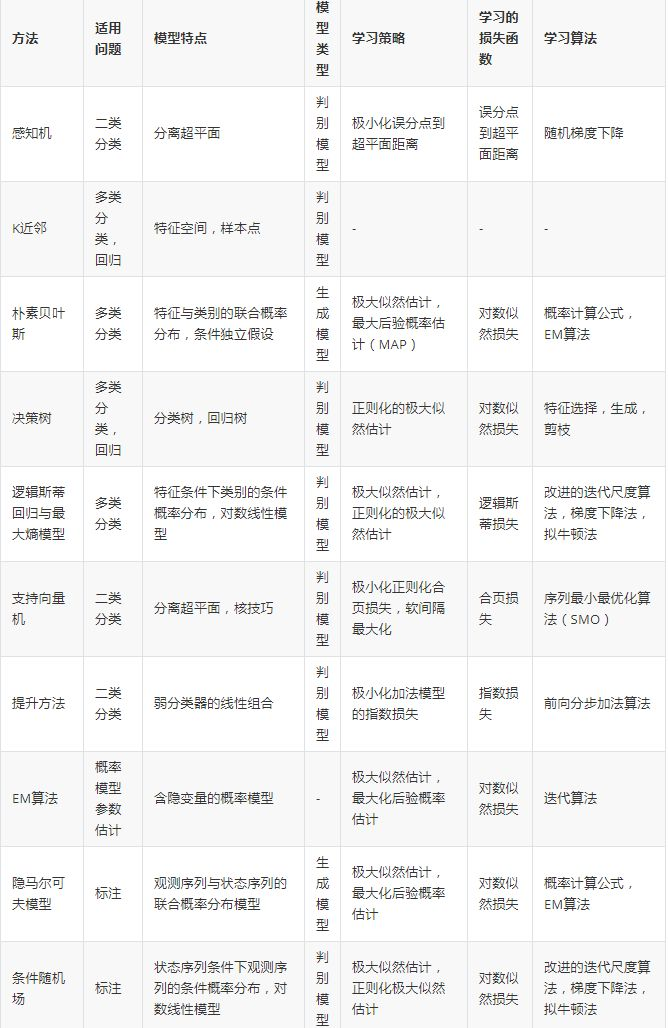
\includegraphics[scale=0.5]{监督学习方法}
		\caption{监督学习方法}
	\end{figure}

\begin{center}
	\textbf{2.无监督学习(Unsupervised Learning)}
\end{center}

又称无导师学习,是指算法根据没有标签的样本来解决各种问题的过程。数据集中的样本只有特征,没有标签,这些标签是模型根据特征按某种规则归纳得出的。具有代表性的是聚类算法和主成分分析PCA。

优点:不需要人参与,训练的数据量可以更大;缺点:难以衡量高维数据的相似性,直观的评价标准还是具有人为的主观性

\begin{center}
	\textbf{3.半监督学习(Semi-Supervised Learning)}
\end{center}

考虑如何利用少量的标注样本和大量的未标注样本进行训练和分类的问题。对于减少标注代价,提高机器学习性能具有非常重大的意义。

半监督学习有三个常用的基本假设:\textbf{平滑假设(Smoothness Assumption),聚类假设(Cluster Assumption),流形假设(Manifold Assumption)}。对于两个样本,如果它们在稠密区域距离很近或者位于同一簇中时,它们的标签很大概率相同。

根据算法模型的结构和功能分类:
\begin{center}
	1.深度学习(Deep Learning)
\end{center}

深层的人工神经网络结构,一种基于数据表征学习的方法,动机在于模拟人脑的分析过程,从底层特征到高层特征一一建模。有前馈神经网络————多层感知机(Multi-Layer Perception,MLP)和卷积神经网络(Convolutional Neural Network,CNN),反馈神经网络————循环神经网络(Recurrent Neural Network,RNN)。

监督学习方法:卷积神经网络,循环卷积网络,多层感知机。无监督学习方法:编码解码器(Encoder-Decoder),生成对抗网络(Generative Adversarial Network,GAN),深度信念网络(Deep Belief Network,DBN),深度玻尔兹曼机(Deep Boltzmann Machine,DBM)

优点:这种结构通过深度的网络不断提取高层次的特征来达到非常优秀的结果。缺点:网络的可解释性不强,训练代价太大,优化困难。
\begin{center}
	2.强化学习(Reinforcement learning)
\end{center}

通过智能体以试错的方式进行学习,不需要真实的标签来指导模型的修改,它是通过智能体不断与环境进行交互来获得奖励或者惩罚,目标是使智能化最终获得的奖励值最大。

深度强化学习(Deep Reinforcement Learning)在解决问题的过程中,强化学习经常会与深度学习相结合,从而使模型获得强大的特征提取和综合能力,
\section{数据预处理}
\subsection{数据清洗}
清洗残缺的数据,错误的数据,重复的数据。数据的清洗工作一般是由计算机完成,而不是人工去除。

步骤:分析数据,残缺数据处理,错误数据处理和重复数据处理。

分析数据:获得数据后,就需要对数据进行统计分析,观察合理数据的大致区间,了解基本的数据信息,找出不合理的数据。

残缺数据处理:

(1)直接删去。适合于缺失数据少,并且缺失数据随机出现,删除对结果影响不大的情况

(2)赋予一个常量。这样的处理效果不好,算法可能会将赋予的常量当作数据本身的属性值。

(3)赋予均值或中位数。对于数据分布正常的数据,可以用均值来赋予;对于数据分布不对称或倾斜的情况,用中位数。

(4)插补法。使用现有未缺失数据通过某种方法来生成该数据。
\\随机插补法:随机选取一个未缺失的值来填充该缺失的部分。
\\热平台插补法:在非缺失的数据中找到一个与缺失样本最相似的样本,使用该样本对缺失的部分进行填充。
\\拉格朗日插值法或牛顿插值法。

(5)建模法。可以使用机器学习中的方法对数据进行建模,然后进行推理预测。比如构造一颗决策树来预测缺失的值。是我们常用的方法。

错误数据判断:

(1)通过简单的数据分析。对于数据其中的属性值一般有个大概的先验感受。利用这种先验来制定某种规则,从而筛选出错误的数据。

(2)3-sigma原则。对于服从正太分布的数据,异常值是那些观测值与均值的偏差超过三倍标准差的数据。

(3)箱型图。通过寻找数据的上四分位值P和下四分位值Q来估计数据大概的上界和下界,那些超过上下界的数据称为异常值。判断错误数据的一种常见方法:由25\%的值可以变得任意远而不会影响四分位值,具有很强的稳定性。
$$upperbound = P+1.5(P-Q)$$
$$lowerbound = Q-1.5(P-Q)$$

(4)建模法。对于不能很好拟合模型的数据,就可以判断为异常值。在了解数据分布的时候,建模的方法效果很好,但是对于高维数据效果可能很差。

(5)基于距离。比较任意两个样本的空间距离,对于那个远离其他样本的样本可以视为离群点。该方法操作简单,但是计算复杂度很高,并且对于多簇分布,数据密度不均匀的情况使用度不高。

(6)基于密度。如果一个样本的局部密度低于它的大部分临近样本的密度,就可视为离群点。

错误数据处理:

(1)直接删去。对于错误数据较少的情况比较适用。

(2)不作处理。算法对于异常值具有很强的鲁棒性就能采用这种方法。

(3)将异常值删去。视为缺省值,并按照缺省值的处理方法进行处理。

重复数据处理:保证数据集中且相同特征的数据只有一份。

直接比较,排序后删除相邻重复数据,使用哈希函数映射后再进行匹配可以提高比较速率,利用集合这种数据结构方便去重。

\subsection{数据集的拆分}
在机器学习中,我们通常将获得的数据集分为三份:
\\(1)训练集(Training Dataset):用来模型迭代训练的数据集。
\\(2)验证集(Validation Dataset):用来预防过拟合的发生,辅助训练过程的数据集。
\\(3)测试集(Test Dataset):用来评估最终训练好的模型性能的数据集。

我们不应该在训练时直接使用训练集来评估训练,不应该将测试集加入到训练集中参与模型的训练。数据划分要注意\textbf{交叉验证(Cross Validation)},可以避免划分训练集和测试集带来的破坏戴数据分布的问题。

划分数据集的方法:

(1)留出法(Hold-Out):选择70\%的样本作为训练集,剩下30\%的样本作为测试集,没有验证集。我们需要多次进行划分,然后重复训练和评估,最后取平均作为最终留出法的评估结果。大数据。

(2)K-折交叉验证法(K-Fold Cross Validation):将原始数据均分为K(K=5,10,20)个互斥的集合,并且尽量每个集合的数据分布保持一致。K组训练集-测试集对,进行K次训练和测试,再通过K次交叉验证取平均得到评估结果。大数据。

(3)自助法(Bootstrap):初始数据集大小为m个样本,每次从数据集中选出一个样本(选出的数据不从原始数据集中删除)放入训练集中。重复进行m次,就得到了m个样本的训练集,最后从原始数据集中选出不在训练集中的那部分样本作为测试集。小数据且难以划分。

一个样本不被选入训练集的概率为$$p=(1-\frac{1}{m})^m$$
当数据集很大时,概率为$$p=\lim_{m \to \infty}(1-\frac{1}{m} )^m=\frac{1}{e}\approx 0.368 $$
\subsection{数据集不平衡}
如果要预测的事件比例小于5\%,那么这样的事件我们称为罕见事件(Rare Event)。处理数据集不平衡的问题的方法有数据层面的重采样,集成算法。

以下处于数据层面的重采样技术主要目标是为了增加少数类的样本数量或者减少多数类的样本数量,从而达到基本平衡。

(1)随机欠采样(Random Under-Sampling):降低多数类参与训练的样本数量,从而使多数类和少数类的样本数量趋于平衡。随机欠采样的优点是减少了训练样本,提高训练的速度;缺点是丢弃了很多可能有用的信息,严重会导致欠采样的数据分布改变。

(2)随机过采样(Random Over-Sampling):通过复制少数类的样本来增加少数类的数量。随机过采样不会丢失有用信息,但是单纯的复制少数类的样本很容易导致过拟合。

(3)基于聚类的过采样(Cluster-Based Over-Sampling):将K-means聚类算法分别用于多数类和少数类样本,然后每一个聚类都被过采样使得所有相同类的聚类都拥有相同数量的样本。

例如:
罪犯群体:2个聚类(20,30) \qquad 非罪犯群体:4个聚类(4000,3000,2000,500)

过采样后:
罪犯群体:2个聚类(2000,2000) \qquad 非罪犯群体:4个聚类(4000,4000,4000,4000)

基于聚类的过采样克服了不同聚类的类间不平衡性,同时也克服了多数类和少数类之间的不平衡性。但是还是有过拟合的可能。

(4)合成少数类过采样技术(Synthetic Minority Over-Sampling Technique,SMOSTE):复制少数类样本与原来的样本做一些改变再加入数据集中。

选取少数类中的若干点,然后对于点A,寻找距离它最近的m个少数类的点,然后从中随机选出一个点B,最后将线段AB连线上的任意一点加入数据集中作为新的少数类点。优点:缓解过拟合问题,不会有信息的丢失。缺点:可能会增加多数类与少数类样本的空间重叠,从而引入额外的噪声,且对高维数据并不有效。

\section{特征工程}
\subsection{特征编码}
不同类型的数据的原始特征(Raw Feature)也不同,我们需要将这些原始特征编码为机器学习算法可使用的类型。

\begin{center}
	1.图像(Image)
\end{center}
一般考虑到图像特征提取过程中产生的中间特征图(Feature Map),有专门的通道数来反映图像中每个像素点的特征向量。因此,图像的原始特征空间大小为$[0,255]^{m\times n\times c}$其中m为图像的高。n为图像的宽,c为图像的通道数。

在传统机器学习算法中,我们一般会将图像的原始特征进行进一步的特征提取,得到高层次的特征后再进行特征的学习,分类等工作。例如:基于图像的行人检测任务,首先对图像提取梯度直方图特征(Histogram of Gradient.HOG),然后再利用支持向量机(Support Vector Machine,SVM)对其中的候选区分类。

\begin{center}
	2.文本(Text)
\end{center}
文本特征是一类需要进行特征编码才能使用的特征。利用One-Hot编码,对于每个文字,我们都通过向量的某一位设置为1来编码,编码的长度为字库的大小。但是当字库非常庞大时特征向量的维度会非常大,会导致维度灾难(维度增加会导致计算量以指数速度增长)。

词嵌入(Word Embedding):将高维的特征向量嵌入到低维空间中,并且映射前后的信息不应该被损失。常用的方法有word2vec。对于两个意思相近的词,它们的距离也应当相近;对于意思不同的词,它们的距离应当远。
\subsection{特征选择与特征降维}
数据降维就是通过特征选择或者特征变换操作将数据从原始的D维空间投影到新的 K 维空间。
\begin{center}
	1.特征选择
\end{center}
特征选择:选择出对模型的预测有用的特征,将那些无用的,有干扰的特征去除的过程。

三种做法(都不易求,变为寻找一个较优的特征子集):
\\(1)无约束的组合优化:从大量特征中选出固定数量的特征,并且使得模型效果最好。
\\(2)有约束的组合优化:对于给定的目标性能,找到数量最小的特征子集。
\\(3)在模型性能和特征数量之间找到一个折中点。

子集搜索(Subset Search):可以通过穷举法尝试所有的特征子集,然后选择最优的结果,但耗时。

为了权衡搜索速度和特征子集的质量,采用\textbf{前向搜索法(Forward Search)}:从空集合开始不断选择当前最优特征。\textbf{反向搜索法(Backward Search)}:从全集开始不断删去无用特征。

\textbf{过滤式(Filter)}:通过信息量或信息增益来衡量特征的有用与无用的程度,然后向空集中加入有用特征或从全集中删除无用特征。

\textbf{包裹式(Wrapper)}:通过后续算法模型的评价指标来衡量当前特征的有用与否,然后向空集中加入有用特征或从全集中删除无用特征。

\textbf{模拟退火算法(Simulated Annealing)}和\textbf{遗传算法(Genetic Algorithm)}通过某种规则随机地寻找优化函数的最优点,但不一定保证是全局最优。
\begin{center}
	2.特征降维
\end{center}

特征降维就是用来减少维度,去除过拟合现象的方法。

\textbf{主成分分析(Principal Component Analysis,PCA)}:一方面可以通过线性变换,降低特征之间的相关性;另一方面我们可以找到主方向(数据差异性最大的方向),主方向的维度对模型的分类是有帮助的。PCA的目的就在于通过一个线性变换,使得变换后的数据方差最大,协方差最小。PCA的本质是将方差最大的方向作为新的主基底(方向),并且在其各个方向上去相关性。

1.对于一组特征${x_1,x_2,...,x_n}$先求出这组特征的中心。$$\bar{x}=\frac{1}{n}\sum_{i=1}^{n}x_i$$

2.对所有特征进行去中心化,并且按行组织成矩阵的形式$$\textbf{X}=[x_1-\bar{x},x_2-\bar{x},...,x_n-\bar{x}]$$

3.再求特征的协方差矩阵(其对角线元素为特征的方差,其他元素为特征间的协方差)$$\textbf{C}=\frac{1}{n}\textbf{X}\textbf{X}^T$$

4.找到线性变换矩阵就是使得协方差矩阵对角化的特征向量,即对协方差矩阵C进行特征分解。$$\textbf{C}=\textbf{VAV}^T$$
对特征值按从大到小排列,最后取前K个最大 的特征值对应的特征向量为新的基底,就组成了所求线性变换的矩阵:$$\textbf{P}=[\textbf{V}^T]_{1:K}$$

\subsection{特征标准化}
由于特征之间的量纲不同,导致每一个特征如果没有归一化完全没有可比性。不经过归一化就进行PCA降维,会筛除掉很多可能有用的特征。
标准化就是一种对样本数据在不同维度上进行一个伸缩变化,但不改变原始数据的分布。好处是在进行特征提取时,忽略不同特征之间的一个度量,而保留样本在各个维度上的信息。其目标在于使不同特征的量纲一致,并且数据变为0至1之间的小数。


1.Min-Max标准化(Min-Max Normalization)又名线性标准化:对原始数据线性变换,使结果值映射到[0,1]之间。

转化函数:
$$
y=\frac{X-min}{max-min}
$$
其中max为样本数据的最大值,min为样本数据的最小值。
这种方法缺陷是当有新数据加入时,可能导致max和min的变化,需重新定义。

线性标准化适用于样本分布比较均匀的情况。

2.标准差标准化方法:给予原始数据的均值(mean)和标准差(standard deviation)进行数据的标准化。经过处理的数据符合标准正态分布,即:均值为0,标准差为1。

转换函数:
$$
y=\frac{X-\mu}{\delta}
$$
其中$\mu$为所有样本数据的均值,$\delta$为所有样本数据的标准差。

适用于样本近似于正太分布,或者当最大值最小值未知,以及在最大最小处存在孤立点的情况

3.Logistic标准化:利用逻辑斯蒂函数进行非线性映射。
$$
y=\frac{1}{1+e^{-x}}
$$

非线性映射用于数据分化比较大的情况
4.反正切函数标准化:利用反正切函数进行非线性映射。
$$y=\frac{arctan(x)\times2}{\pi}$$

5.小数定标标准化:直接移动小数点位置来实现标准化,其中j是使得最大的y小于1的最小值。
$$y=\frac{x}{10^j}$$
\section{模型评估}
\begin{center}
	1.回归问题
\end{center}
评价指标会选择:平均平方误差,平均绝对误差,平均对数误差
\begin{center}
	2.分类问题
\end{center}
需要得到类别c预测结果的混淆矩阵:
\begin{table}[htbp]
	\centering
	\scalebox{1}{
	\begin{tabular}{|c|c|c|c|}
		\hline
		\multirow{4}{*}{真实类别} & \multirow{2}{*}{y值}     & \multicolumn{2}{c|}{预测类别}                                                  \\ \cline{3-4} 
		&                         & $\hat{y}$=c & $\hat{y}\neq c$ \\ \cline{2-4} 
		& y=c                     & TP                         & FN                                            \\ \cline{2-4} 
		& y $\neq$ c & FP                         & TN                                            \\ \hline
	\end{tabular}}
\end{table}
\textbf{真正例(True Positive,TP)}:真实类别为c且预测结果也为c的样本。
\textbf{假负例(False Negative,FN)}:又称假阴性样本,真实类别为c却预测为其他类别的样本。
\textbf{假正例(False Positive,FP)}:又称假阳性样本,真实类别不为c却预测为类别c的样本。
\textbf{真负例(True Negatuve,TN)}:真实类别不为c且预测结果也不为c的样本。

\textbf{准确率(Accuracy)}:衡量分类结果的正确性。
$$Accuracy=\frac{1}{N}\sum_{i=1}^{N}I(y_i=\hat{y}_i)=\frac{TP+TN}{TP+FN+FP+TN}$$

\textbf{错误率(Error Rate)}:衡量分类结果的错误性。
$$ErrorRate=1-Accuracy=\frac{1}{N}\sum_{i=1}^{N}I(y_i\neq \hat{y}_i)=\frac{FN+FP}{TP+FN+FP+TN}$$

\textbf{查准率(Precision)}:精确度或精度,代表的预测为类别c的样本中有多少预测正确了。
$$Precision = \frac{TP}{TP+FP}$$

\textbf{查全率(Recall)}:召回率,代表真实标签为类别c的众多样本中,有多少被真正检测出来了。
$$Recall = \frac{TP}{TP+FN}$$

\textbf{F值(F Measure)}:综合查准率和查全率两者关系的一个综合性指标。
$$F=\frac{(1+\beta^2)\bullet Precision\bullet Recall}{\beta^2 \bullet Precision + Recall}$$
其中$\beta$值用于平衡准确率和查全率(两者一般不可以兼得),一般取值为1,称为F值。

\textbf{宏平均(Macro Average)}:用于计算每一类别整体的精确率,召回率和F1值的算术平均值和\textbf{微平均(Micro Average)}:计算每一个样本的精确率,召回率和F1值的算术平均值。使用宏平均更合理。
$$Precision_{macro}=\frac{1}{C}\sum_{c=1}^{C}Precision_c$$
$$Recall_{macro}=\frac{1}{C}\sum_{c=1}^{C}Recall$$
$$F1_{macro}=\frac{2\bullet Procision_{macro}\bullet Recall_{macro}}{Precision_{macro}+Recall_{macro}}$$

\section{鸢尾花分类代码实现}
\begin{Python}{代码实现}
import numpy as np
from matplotlib import colors
from sklearn import svm
from sklearn.svm import SVC
from sklearn import model_selection
import matplotlib.pyplot as plt
import matplotlib as mpl

def iris_type(s):
	it = {b'Iris-setosa':0, b'Iris-versicolor':1, b'Iris-virginica':2}
	return it[s]

#加载数据
data_path='D:\python_code\dataset\iris.data'          #数据文件的路径
data = np.loadtxt(data_path,                                #数据文件路径
				  dtype=float,                              #数据类型
				  delimiter=',',                            #数据分隔符
				  converters={4:iris_type})                 #将第5列使用函数iris_type进行转换
#print(data)                                                #data为二维数组,data.shape=(150, 5)
#print(data.shape)
#数据分割
x, y = np.split(data,                                       #要切分的数组
				(4,),                                       #沿轴切分的位置,第5列开始往后为y
				axis=1)                                     #代表纵向分割,按列分割
x = x[:, 0:2]                                            #在X中我们取前两列作为特征,为了后面的可视化。x[:,0:2]代表第一维(行)全取,第二维(列)取0~2
#print(x)
x_train,x_test,y_train,y_test=model_selection.train_test_split(
						x,              #所要划分的样本特征集
						y,              #所要划分的样本结果
						random_state=1, #随机数种子
						test_size=0.3)  #测试样本占比
#**********************SVM分类器构建*************************
def classifier():
	#clf = svm.SVC(C=0.8,kernel='rbf', gamma=50,decision_function_shape='ovr')
	clf = svm.SVC(C=0.5,                         #误差项惩罚系数,默认值是1
				  kernel='linear',               #线性核 kenrel="rbf":高斯核
				  decision_function_shape='ovr') #决策函数
	return clf
# 2.定义模型:SVM模型定义
clf = classifier()
#***********************训练模型*****************************
def train(clf,x_train,y_train):
	clf.fit(x_train,         #训练集特征向量
			y_train.ravel()) #训练集目标值
# 3.训练SVM模型
train(clf,x_train,y_train)
#**************并判断a b是否相等,计算acc的均值*************
def show_accuracy(a, b, tip):
	acc = a.ravel() == b.ravel()
	print('%s Accuracy:%.3f' %(tip, np.mean(acc)))
def print_accuracy(clf,x_train,y_train,x_test,y_test):
	#分别打印训练集和测试集的准确率  score(x_train,y_train):表示输出x_train,y_train在模型上的准确率
	print('trianing prediction:%.3f' %(clf.score(x_train, y_train)))
	print('test data prediction:%.3f' %(clf.score(x_test, y_test)))
	#原始结果与预测结果进行对比   predict()表示对x_train样本进行预测,返回样本类别
	show_accuracy(clf.predict(x_train), y_train, 'traing data')
	show_accuracy(clf.predict(x_test), y_test, 'testing data')
	#计算决策函数的值,表示x到各分割平面的距离
	print('decision_function:\n', clf.decision_function(x_train))
# 4.模型评估
print_accuracy(clf,x_train,y_train,x_test,y_test)

def draw(clf, x):
	iris_feature = 'sepal length', 'sepal width', 'petal lenght', 'petal width'
	# 开始画图
	x1_min, x1_max = x[:, 0].min(), x[:, 0].max()  # 第0列的范围
	x2_min, x2_max = x[:, 1].min(), x[:, 1].max()  # 第1列的范围
	x1, x2 = np.mgrid[x1_min:x1_max:200j, x2_min:x2_max:200j]  # 生成网格采样点
	grid_test = np.stack((x1.flat, x2.flat), axis=1)  # stack():沿着新的轴加入一系列数组
	print('grid_test:\n', grid_test)
	# 输出样本到决策面的距离
	z = clf.decision_function(grid_test)
	print('the distance to decision plane:\n', z)
	grid_hat = clf.predict(grid_test)  # 预测分类值 得到【0,0.。。。2,2,2】
	print('grid_hat:\n', grid_hat)
	grid_hat = grid_hat.reshape(x1.shape)  # reshape grid_hat和x1形状一致
	# 若3*3矩阵e,则e.shape()为3*3,表示3行3列
	cm_light = mpl.colors.ListedColormap(['#A0FFA0', '#FFA0A0', '#A0A0FF'])
	cm_dark = mpl.colors.ListedColormap(['g', 'r', 'b'])
	plt.pcolormesh(x1, x2, grid_hat, cmap=cm_light)  # pcolormesh(x,y,z,cmap)这里参数代入
	# x1,x2,grid_hat,cmap=cm_light绘制的是背景。
	plt.scatter(x[:, 0], x[:, 1], c=np.squeeze(y), edgecolor='k', s=50, cmap=cm_dark)  # 样本点
	plt.scatter(x_test[:, 0], x_test[:, 1], s=120, facecolor='none', zorder=10)  # 测试点
	plt.xlabel(iris_feature[0], fontsize=20)
	plt.ylabel(iris_feature[1], fontsize=20)
	plt.xlim(x1_min, x1_max)
	plt.ylim(x2_min, x2_max)
	plt.title('svm in iris data classification', fontsize=30)
	plt.grid()
	plt.show()

# 5.模型使用
draw(clf,x)
\end{Python}
\begin{figure}[htbp]
	\centering
	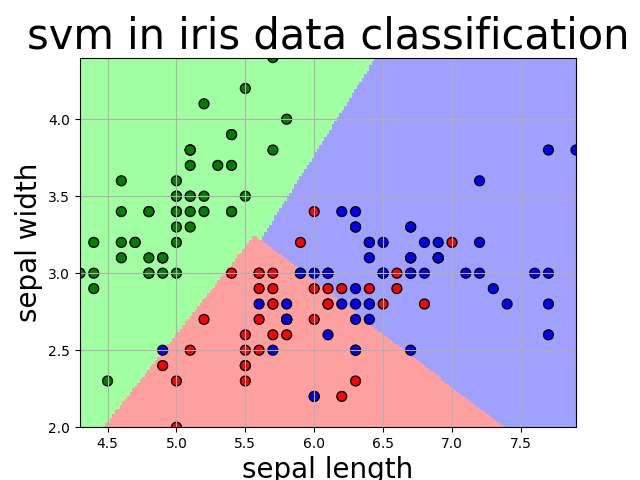
\includegraphics[scale=0.38]{Figure_1}
\end{figure}
\end{document}

极地反击,